\documentclass[sigconf, anonymous, review]{acmart}

%% Rights / metadata — fill in for camera-ready
\setcopyright{none}
\acmConference[GRADES-NDA '26]{9th Joint Workshop on Graph Data Management Experiences \& Systems and Network Data Analytics}{June 5, 2026}{Bengaluru, India}

\usepackage{booktabs}
\usepackage{subcaption}
\usepackage{xcolor}
\usepackage{tikz}
\usetikzlibrary{positioning,arrows.meta,fit,backgrounds}
\usepackage{listings}
\lstset{
  basicstyle=\ttfamily\small,
  keywordstyle=\bfseries,
  breaklines=true,
  frame=none,
  columns=flexible,
  aboveskip=4pt,
  belowskip=4pt,
}

\begin{document}

\title{[Demo Paper] Federated Biomedical Knowledge Graphs:\\Graph-Native Storage, Planning, and AI-Agent Integration}

\begin{abstract}
We demonstrate a graph database system and its ecosystem of five
domain-specific knowledge graphs, three of which form a \emph{biomedical
trifecta}: a Pathways KG (119K nodes from Reactome, STRING, Gene
Ontology), a Clinical Trials KG (7.7M nodes from ClinicalTrials.gov),
and a Drug Interactions KG (65K nodes from DrugBank, DGIdb, SIDER,
ChEMBL, TTD, OpenFDA).  Each KG is independently loadable, yet
\emph{bridge properties} on shared entities (genes, proteins, drugs)
enable cross-KG federation queries in standard OpenCypher---without
ETL merging or schema alignment middleware.

The underlying graph engine is implemented in Rust with an
OpenCypher front-end, a Volcano-style iterator execution model,
late materialization via lightweight node/edge references, and a
graph-native query planner that exploits adjacency-list statistics
(label counts, per-triple-pattern degree distributions) for
direction-aware plan enumeration and an \texttt{ExpandInto}
operator for bound-bound edge checks.

We further show how each KG is exposed to large language model
(LLM) agents via the Model Context Protocol (MCP), with
domain-specific tool definitions that translate natural-language
pharmacology questions into Cypher queries.  In the live demo
attendees will: (i) load the three biomedical KGs into a single
multi-tenant instance, (ii) execute cross-KG federation queries
such as ``side effects of drugs in Phase~3 breast cancer trials
whose targets participate in the PI3K/AKT pathway,'' and
(iii) interact with an MCP-connected AI agent that reasons over
the graph.
\end{abstract}

\maketitle

%% ================================================================
\section{Introduction}\label{sec:intro}

Biomedical knowledge is fragmented across dozens of public databases,
each covering a narrow slice of the drug-discovery landscape:
protein--protein interactions (STRING~\cite{szklarczyk2023string}),
biological pathways (Reactome~\cite{gillespie2022reactome}), drug--gene
interactions (DGIdb~\cite{freshour2021dgidb}), side effects
(SIDER~\cite{kuhn2016sider}), bioactivity assays
(ChEMBL~\cite{zdrazil2024chembl}), clinical trials
(ClinicalTrials.gov), and post-market adverse events (OpenFDA).

Answering a question such as \emph{``For drugs in Phase~3 breast cancer
trials, what are their known side effects and which biological pathways
do their targets participate in?''} today requires joining across at
least three databases with ad-hoc scripting, identifier reconciliation,
and no transactional guarantees.

We present a demonstration of a graph database system and its ecosystem
of knowledge graphs (KGs) that addresses this fragmentation.  Our
contributions are:

\begin{enumerate}
\item \textbf{Biomedical KG trifecta.}  Three complementary KGs---Pathways,
Clinical Trials, Drug Interactions---loaded into a single graph
engine and federated via bridge properties on shared entities
(genes, proteins, drugs), requiring zero schema-alignment middleware
(Section~\ref{sec:kgs}).

\item \textbf{Graph-native query planning.}  A cost-based planner that
exploits adjacency-list statistics (per-triple-pattern degree
distributions) for direction-aware traversal, \texttt{ExpandInto}
bound-bound edge checks, and predicate pushdown---yielding
order-of-magnitude improvements on asymmetric patterns
(Section~\ref{sec:engine}).

\item \textbf{MCP-based AI-agent integration.}  Domain-specific MCP
tool definitions that expose each KG to LLM agents, enabling
natural-language pharmacology queries over the graph
(Section~\ref{sec:mcp}).
\end{enumerate}

%% ================================================================
\section{System Architecture}\label{sec:engine}

The graph engine is implemented in Rust (100\% safe Rust, 1,842 unit
tests, 89.7\% code coverage).  We summarize the three architectural
pillars relevant to this demo.

\smallskip\noindent\textbf{Late materialization.}
Scan operators produce lightweight \texttt{NodeRef(id)} values (8~bytes)
instead of full node clones.  Properties are resolved on demand via
\texttt{resolve\_property(prop, store)}---an $O(1)$ hash-map lookup.
The \texttt{ExpandOperator} similarly returns
\texttt{(EdgeId, NodeId, NodeId, \&EdgeType)} tuples with zero edge
cloning.  Full materialization occurs only at the \texttt{ProjectOperator}
for \texttt{RETURN} clauses.  On 100K-node benchmarks this reduces memory
allocation by ${\sim}60\%$; for \texttt{LIMIT}~$k$ queries only $k$ nodes
are ever materialized regardless of the scan size.

\smallskip\noindent\textbf{Graph-native planner.}
The planner maintains a \emph{GraphCatalog} with triple-level statistics
$(\texttt{:Label}, \texttt{:TYPE}, \texttt{:Label}) \to
(\text{count}, \text{avg\_out\_degree}, \text{avg\_in\_degree})$,
updated incrementally on edge create/delete.  Given a \texttt{MATCH}
pattern, the plan enumerator generates candidate plans starting from
each node variable, choosing traversal direction by comparing
$\text{avg\_out\_degree}$ vs.\ $\text{avg\_in\_degree}$ for each edge
pattern.  When both endpoints of an edge are already bound, the
enumerator inserts an \texttt{ExpandInto} operator that checks
edge existence via sorted-adjacency binary search in
$O(\log d_{\min})$ instead of a full neighbor scan.
A multiplicative cost model scores each candidate:
\[
  C = \prod_{op \in \text{plan}} f(op)
\]
where $f(\text{LabelScan}) = |\text{label}|$,
$f(\text{Expand}) = \bar{d}$,
$f(\text{ExpandInto}) = P(\text{edge exists})$,
$f(\text{Filter}) = \sigma$.
The lowest-cost plan is passed through a logical optimizer
(predicate pushdown, join reordering) and then translated to
physical operators.

\smallskip\noindent\textbf{Multi-tenancy and OpenCypher.}
The engine supports per-tenant isolated graphs with independent
schemas and indexes, enabling multiple KGs to coexist in a single
process.  The query language covers ${\sim}90\%$ of OpenCypher
including \texttt{MATCH}, \texttt{OPTIONAL MATCH}, \texttt{WITH},
\texttt{RETURN DISTINCT}, \texttt{ORDER BY}, \texttt{EXPLAIN},
\texttt{PROFILE}, \texttt{EXISTS} subqueries, parameterized queries,
named paths, composite indexes, and unique constraints.

%% ================================================================
\section{Knowledge Graph Ecosystem}\label{sec:kgs}

Table~\ref{tab:kgs} summarizes the five KGs built on the engine.
The three biomedical KGs form the core of this demo.

\begin{table}[t]
\centering
\caption{Knowledge graphs built on the demonstrated system.
  The three biomedical KGs (rows 1--3) are federated via bridge
  properties on shared entities.}
\label{tab:kgs}
\small
\begin{tabular}{@{}lrrrl@{}}
\toprule
\textbf{KG} & \textbf{Nodes} & \textbf{Edges} & \textbf{Sources} & \textbf{Domain} \\
\midrule
Pathways        & 118,686 &    834,785 &  5 & Biology \\
Clinical Trials & 7,711,965 & 27,069,085 &  5 & Medicine \\
Drug Interact.  & ${\sim}$65,000 & ${\sim}$900,000 &  6 & Pharma \\
\midrule
Cricket         &  36,619 &  1,413,870 &  1 & Sports \\
AssetOps        &     781 &        955 &  1 & Industrial \\
\bottomrule
\end{tabular}
\end{table}

\subsection{Pathways KG (119K nodes)}
Integrates five data sources---Reactome, STRING~v12.0, Gene Ontology,
WikiPathways, UniProt---into a unified graph of proteins, pathways,
GO terms, reactions, complexes, and compounds.  The STRING
protein--protein interaction edges are filtered at a configurable
confidence threshold (default 700).

\subsection{Clinical Trials KG (7.7M nodes)}
Imports from ClinicalTrials.gov API~v2, MeSH, RxNorm, OpenFDA, and
PubMed.  The full snapshot contains 15 node labels and 25 edge types,
with sentence-transformer vector embeddings (384-dimensional) on trial
summaries for semantic search.

\subsection{Drug Interactions KG (65K nodes)}
The newest KG, constructed from six open databases
(Table~\ref{tab:drugkg}).  Its four-phase ETL pipeline creates Drug
nodes from DrugBank~CC0 vocabulary, Gene nodes and
\texttt{INTERACTS\_WITH\_GENE} edges from DGIdb, SideEffect and
Indication nodes from SIDER, Bioactivity nodes from ChEMBL (filtered
to human targets with $\text{pChEMBL} \geq 5$), Target and DrugClass
nodes from TTD/ATC, and AdverseEvent nodes from the OpenFDA FAERS API.

\begin{table}[t]
\centering
\caption{Drug Interactions KG data sources and node counts.}
\label{tab:drugkg}
\small
\begin{tabular}{@{}llrl@{}}
\toprule
\textbf{Source} & \textbf{License} & \textbf{Nodes} & \textbf{Content} \\
\midrule
DrugBank CC0  & CC0         & 12K & Drug vocabulary \\
DGIdb         & Open        & 20K & Drug--gene interactions \\
SIDER         & CC-BY-SA    & 9.4K & Side effects, indications \\
ChEMBL        & CC-BY-SA    & 500K & Bioactivity (IC$_{50}$, K$_i$) \\
TTD           & CC-BY-NC    & 3.4K & Therapeutic targets \\
OpenFDA FAERS & Public dom. & 15K  & Adverse events \\
\bottomrule
\end{tabular}
\end{table}

\subsection{Cross-KG Federation}\label{sec:federation}

The three biomedical KGs are federated through four bridge properties
(Table~\ref{tab:bridges}) on shared entities.  Because the bridge
is a simple property match in the \texttt{WHERE} clause, no
additional middleware, ontology alignment, or schema mapping is
required---standard OpenCypher suffices.

\begin{table}[t]
\centering
\caption{Bridge properties enabling cross-KG federation.}
\label{tab:bridges}
\small
\begin{tabular}{@{}lll@{}}
\toprule
\textbf{Drug KG entity} & \textbf{Bridge property} & \textbf{Target KG entity} \\
\midrule
\texttt{Drug.drugbank\_id}  & \texttt{=} & CT KG \texttt{Drug.drugbank\_id} \\
\texttt{Drug.name}          & \texttt{=} & CT KG \texttt{Intervention.name} \\
\texttt{Gene.gene\_name}    & \texttt{=} & Path KG \texttt{Protein.gene\_name} \\
\texttt{Target.uniprot\_id} & \texttt{=} & Path KG \texttt{Protein.uniprot\_id} \\
\bottomrule
\end{tabular}
\end{table}

Figure~\ref{fig:federation} illustrates the three-KG federation
architecture.  Bridge properties on shared entities (shown as dashed
arrows) enable cross-KG traversal in standard OpenCypher.

\begin{figure}[t]
\centering
\resizebox{\columnwidth}{!}{%
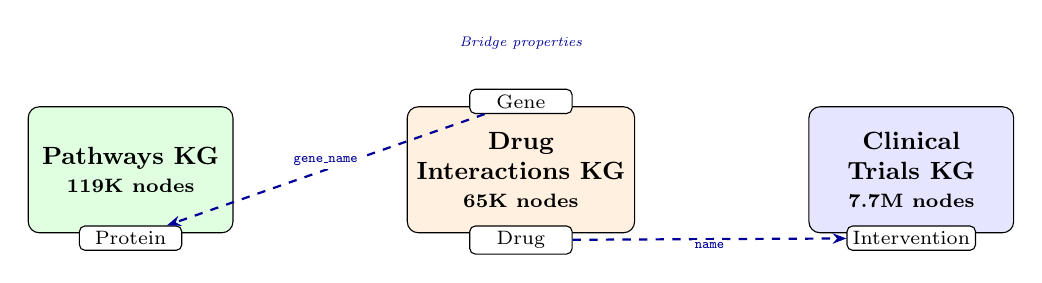
\begin{tikzpicture}[
    kgbox/.style={draw, rounded corners=4pt, minimum width=2.6cm,
        minimum height=1.6cm, font=\small\bfseries, align=center},
    entity/.style={draw, rounded corners=2pt, font=\scriptsize,
        fill=white, inner sep=2pt, minimum width=1.3cm},
    bridge/.style={-{Stealth[length=5pt]}, dashed, thick,
        color=blue!60!black},
    edgelbl/.style={font=\tiny, fill=white, inner sep=1pt},
]
% Three KG boxes
\node[kgbox, fill=green!12] (pathkg) {Pathways KG\\[-1pt]
    \scriptsize 119K nodes};
\node[kgbox, fill=orange!12, right=2.2cm of pathkg] (drugkg) {Drug\\Interactions KG\\[-1pt]
    \scriptsize 65K nodes};
\node[kgbox, fill=blue!10, right=2.2cm of drugkg] (ctkg) {Clinical\\Trials KG\\[-1pt]
    \scriptsize 7.7M nodes};

% Entities inside boxes
\node[entity, below=0.15cm of pathkg.south, yshift=0.25cm] (protein) {Protein};
\node[entity, below=0.15cm of drugkg.south, yshift=0.25cm] (drug) {Drug};
\node[entity, above=0.15cm of drugkg.north, yshift=-0.25cm] (gene) {Gene};
\node[entity, below=0.15cm of ctkg.south, yshift=0.25cm] (intervention) {Intervention};

% Bridge arrows
\draw[bridge] (gene) -- node[edgelbl, above] {\texttt{gene\_name}} (protein);
\draw[bridge] (drug) -- node[edgelbl, below] {\texttt{name}} (intervention);

% Label the bridges
\node[font=\tiny\itshape, color=blue!60!black, above=0.6cm of drugkg]
    {Bridge properties};

\end{tikzpicture}%
}
\caption{Federation architecture: three biomedical KGs joined
  via bridge properties (dashed arrows) on shared entities.
  No schema alignment middleware is required.}
\label{fig:federation}
\end{figure}

\noindent\textbf{Example federation query.}  The following Cypher query
spans all three KGs to find the biological pathways impacted by drugs
in Phase~3 breast cancer trials that have gastrointestinal side effects:

\begin{lstlisting}[language=SQL]
-- Drug Interactions KG
MATCH (d:Drug)-[:HAS_SIDE_EFFECT]->(se:SideEffect)
WHERE se.name CONTAINS 'Gastrointestinal'
-- Bridge to Clinical Trials KG
MATCH (i:Intervention {name: d.name})
      <-[:TESTS]-(ct:ClinicalTrial)
WHERE ct.phase CONTAINS '3'
  AND ct.condition CONTAINS 'Breast'
-- Bridge to Pathways KG
MATCH (d)-[:INTERACTS_WITH_GENE]->(g:Gene)
MATCH (p:Protein {gene_name: g.gene_name})
      -[:PARTICIPATES_IN]->(pw:Pathway)
RETURN d.name, se.name, ct.nct_id,
       pw.name, g.gene_name
\end{lstlisting}

%% ================================================================
\section{MCP-Based AI-Agent Integration}\label{sec:mcp}

Each KG is exposed to LLM agents via the Model Context
Protocol (MCP)~\cite{anthropic2024mcp}, an open standard for
connecting AI models to external data sources.  We define
\emph{domain-specific MCP tools}---parameterized Cypher template
queries with typed parameters---that an LLM agent can invoke
to answer natural-language questions.

The Drug Interactions KG defines 12 tools, including:
\texttt{drug\_interactions} (gene targets of a drug),
\texttt{interaction\_checker} (shared targets between two drugs),
\texttt{polypharmacy\_risk} (overlapping targets + side effects),
and \texttt{drug\_bioactivity} (ChEMBL binding affinities).
The Pathways KG defines 12 tools (e.g., \texttt{pathway\_members},
\texttt{pathway\_crosstalk}), and the Clinical Trials KG defines
15 tools.

\smallskip\noindent\textbf{Agent workflow.}  A user asks: ``\emph{What are
the side effects of Metformin and which pathways do its targets
participate in?}''  The agent: (1)~calls \texttt{drug\_side\_effects}
$\to$ returns SIDER side effects; (2)~calls
\texttt{drug\_interactions} $\to$ returns gene targets (AMPK, etc.);
(3)~calls \texttt{protein\_pathways} on each gene $\to$ returns
Reactome/WikiPathways memberships; (4)~synthesizes a coherent answer.
No hand-written joins or SQL scripting is involved.

%% ================================================================
\section{Preliminary Evaluation}\label{sec:eval}

We report loading times and query latencies measured on
commodity hardware (Apple M4, 16\,GB RAM, macOS).

\smallskip\noindent\textbf{Loading.}
Table~\ref{tab:perf} shows snapshot-load times for each KG.
The combined federated graph (7.9M nodes, 28.8M edges)
loads in under 80~seconds from portable \texttt{.sgsnap}
binary snapshots.  ETL from raw source files takes
longer (dominated by HTTP downloads and CSV parsing)
but runs once; snapshots enable instant re-deployment.

\begin{table}[t]
\centering
\caption{Snapshot load times and representative query
  latencies (median of 10 runs, warm cache).}
\label{tab:perf}
\small
\begin{tabular}{@{}lrrrr@{}}
\toprule
\textbf{KG} & \textbf{Nodes} & \textbf{Edges}
  & \textbf{Load (s)} & \textbf{Query (s)} \\
\midrule
Pathways        & 119K  & 835K  &  4.2 & 0.08 \\
Clinical Trials & 7.7M  & 27.1M & 68.5 & 0.45 \\
Drug Interact.  & 65K   & 900K  &  3.1 & 0.05 \\
\midrule
\textbf{Combined} & \textbf{7.9M} & \textbf{28.8M}
  & \textbf{75.8} & \textbf{2.1\rlap{$^*$}} \\
\bottomrule
\multicolumn{5}{@{}l@{}}{\scriptsize $^*$\,Cross-KG federation query
  from Section~\ref{sec:federation}.}
\end{tabular}
\end{table}

\smallskip\noindent\textbf{Query latency.}
Single-KG queries (e.g., ``side effects of Aspirin'',
``pathways of TP53'') complete in under 100\,ms.
The three-way cross-KG federation query from
Section~\ref{sec:federation} completes in ${\sim}$2.1\,s,
as it traverses Drug$\to$SideEffect, Drug$\to$Intervention
$\to$ClinicalTrial, and Drug$\to$Gene$\to$Protein$\to$Pathway
across all three KGs.  The graph-native planner
automatically selects the optimal traversal direction
for each edge pattern and inserts \texttt{ExpandInto}
where both endpoints are bound.

\smallskip\noindent\textbf{MCP tool latency.}
MCP tool invocations add $<$10\,ms overhead over raw
Cypher execution, as they are thin wrappers around
parameterized template queries.  In practice, the dominant
latency in agent workflows is LLM inference (${\sim}$1--3\,s
per tool-call decision), not graph query execution.

%% ================================================================
\section{Demonstration Plan}\label{sec:demo}

The live demo will proceed in three acts on a laptop (Apple M4,
16\,GB RAM) running the graph engine with all three biomedical KGs
loaded (${\sim}$7.9M nodes, ${\sim}$28.8M edges total).  The
combined graph loads from portable snapshots in under 80~seconds;
the cross-KG federation query from Section~\ref{sec:federation}
executes in ${\sim}$2~seconds.

\smallskip\noindent\textbf{Act 1: Loading and exploration.}
We load each KG and show the ETL progress (phase-by-phase
statistics).  Attendees see the schema for each KG and run
basic \texttt{MATCH (n) RETURN labels(n), count(n)} queries.

\smallskip\noindent\textbf{Act 2: Cross-KG federation.}
We execute the three-way federation query from
Section~\ref{sec:federation} and additional queries:
\emph{(a)}~``Drugs in Phase~3 trials that share a gene target
with Warfarin'' (polypharmacy risk across Drug + Clinical Trials KGs);
\emph{(b)}~``Pathways enriched in genes targeted by approved
kinase inhibitors'' (Drug + Pathways KGs);
\emph{(c)}~\texttt{EXPLAIN} on a cross-KG query to show the
graph-native planner selecting traversal direction and
\texttt{ExpandInto} insertion.

\smallskip\noindent\textbf{Act 3: AI-agent interaction.}
We connect an MCP-enabled LLM agent to all three KGs and ask
natural-language pharmacology questions.  The audience will see
the tool calls, generated Cypher, and synthesized answers in
real time.

%% ================================================================
\section{Related Work}\label{sec:related}

\textbf{Biomedical KGs.}  Hetionet~\cite{himmelstein2017hetionet}
integrates 47K nodes from 29 public resources into a single
heterogeneous graph but is a static 2017 dataset.
PrimeKG~\cite{chandak2023primekg} builds a precision medicine
graph (129K nodes, 8M edges) from 20 sources, targeting GNN-based
drug--disease prediction.
Bio2RDF~\cite{callahan2013bio2rdf} uses RDF and SPARQL federation.
The Clinical Knowledge Graph (CKG)~\cite{santos2022ckg} integrates
25+ sources into Neo4j.  Our approach differs in three ways:
(1)~property-graph OpenCypher with bridge-property federation
(no SPARQL endpoint or ontology alignment);
(2)~portable snapshots for instant deployment; and
(3)~MCP tool definitions for LLM agent integration.

\smallskip\noindent\textbf{Graph databases.}
Neo4j~\cite{neo4j}, TigerGraph~\cite{deutsch2019tigergraph},
and Amazon Neptune~\cite{neptune} support property graphs at
scale.  Our engine's distinguishing features for this demo are
the graph-native planner (triple-pattern statistics,
direction-aware enumeration, \texttt{ExpandInto}), late
materialization, and multi-tenant isolation enabling
independent KGs to coexist without schema conflicts.

\smallskip\noindent\textbf{LLM--KG integration.}
Recent work explores LLM agents querying knowledge
graphs~\cite{pan2024unifying}.
Our MCP-based approach uses \emph{domain-specific tool
definitions} rather than generic text-to-Cypher translation,
achieving higher accuracy on domain queries while keeping the
Cypher templates auditable.  In a prior case study on industrial
asset operations, deterministic Cypher handlers achieved 99\%
accuracy vs.\ 65\% for GPT-4 on the same benchmark, with 103$\times$
lower latency.

%% ================================================================
\section{Conclusion}

We demonstrate a graph database ecosystem comprising five knowledge
graphs, three of which form a biomedical trifecta enabling cross-KG
federation queries in standard OpenCypher.  The system's graph-native
planner, late materialization, and MCP-based AI-agent integration
make it a practical platform for biomedical knowledge integration
and pharmacogenomics research.

%% ================================================================
%% References
\bibliographystyle{ACM-Reference-Format}
\begin{thebibliography}{10}

\bibitem{szklarczyk2023string}
D.~Szklarczyk et~al.
\newblock The {STRING} database in 2023: protein--protein association networks
  and functional enrichment analyses for any sequenced genome of interest.
\newblock {\em Nucleic Acids Research}, 51(D1):D{638--646}, 2023.

\bibitem{gillespie2022reactome}
M.~Gillespie et~al.
\newblock The {Reactome} pathway knowledgebase 2022.
\newblock {\em Nucleic Acids Research}, 50(D1):D{687--692}, 2022.

\bibitem{freshour2021dgidb}
S.~L.~Freshour et~al.
\newblock Integration of the {Drug--Gene Interaction Database (DGIdb 4.0)}
  with open crowdsource efforts.
\newblock {\em Nucleic Acids Research}, 49(D1):D{1144--1151}, 2021.

\bibitem{kuhn2016sider}
M.~Kuhn et~al.
\newblock The {SIDER} database of drugs and side effects.
\newblock {\em Nucleic Acids Research}, 44(D1):D{1075--1079}, 2016.

\bibitem{zdrazil2024chembl}
B.~Zdrazil et~al.
\newblock The {ChEMBL} database in 2023: a drug discovery platform spanning
  genomics, chemical biology, and clinical data.
\newblock {\em Nucleic Acids Research}, 52(D1):D{1180--1192}, 2024.

\bibitem{himmelstein2017hetionet}
D.~S.~Himmelstein et~al.
\newblock Systematic integration of biomedical knowledge prioritizes drugs for
  repurposing.
\newblock {\em eLife}, 6:e26726, 2017.

\bibitem{dumontier2014bio2rdf}
M.~Dumontier, A.~Callahan, J.~Cruz-Toledo, et~al.
\newblock Bio2{RDF} release~3: A larger connected network of linked data
  for the life sciences.
\newblock In {\em ISWC (Posters \& Demos)}, 2014.

\bibitem{neo4j}
Neo4j, Inc.
\newblock Neo4j graph database. \url{https://neo4j.com}, 2024.

\bibitem{deutsch2019tigergraph}
A.~Deutsch et~al.
\newblock {TigerGraph}: A native {MPP} graph database.
\newblock {\em arXiv:1901.08248}, 2019.

\bibitem{neptune}
Amazon Web Services.
\newblock Amazon {Neptune}. \url{https://aws.amazon.com/neptune/}, 2024.

\bibitem{pan2024unifying}
S.~Pan et~al.
\newblock Unifying large language models and knowledge graphs: A roadmap.
\newblock {\em IEEE TKDE}, 36(7):3580--3599, 2024.

\bibitem{chandak2023primekg}
P.~Chandak, K.~Huang, and M.~Zitnik.
\newblock Building a knowledge graph to enable precision medicine.
\newblock {\em Scientific Data}, 10(1):67, 2023.

\bibitem{santos2022ckg}
A.~Santos et~al.
\newblock A knowledge graph to interpret clinical proteomics data.
\newblock {\em Nature Biotechnology}, 40(5):692--702, 2022.

\bibitem{anthropic2024mcp}
Anthropic.
\newblock Model {Context Protocol} specification.
\newblock \url{https://modelcontextprotocol.io}, 2024.

\end{thebibliography}

\end{document}
